\documentclass{standalone}
\usepackage{tikz}

\usetikzlibrary{intersections}

\begin{document}
	
	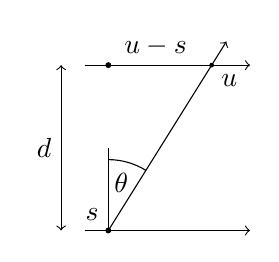
\begin{tikzpicture}[scale = 0.3, baseline]
	
		\draw[->] (-1, 0) -- (6, 0);
		\draw[name path=uAxis, ->] (-1, 7) -- (6, 7);
		
		\draw[name path=ray, ->] (0, 0) -- (5, 8);
		\node[above left] {$s$};
		
		\draw[fill] (0, 0) circle [radius = 0.1];
		\draw[fill] (0, 7) circle [radius = 0.1];
		
		\fill[name intersections={of=uAxis and ray, total=\t}]
		\foreach \s in {1,...,\t}{(intersection-\s) circle[radius = 0.1] node[below right] {$u$}};
		
		\draw (0, 0) -- (0, 3.5);
		\draw (0, 3) arc (90 : 90 - atan(5/8) : 3);
		\node at (0.55, 2) {$\theta$};
		
		\node[above] at (2, 7) {$u - s$};
		
		\draw[<->] (-2, 0) -- (-2, 7);
		\node[left] at (-2, 3.5) {$d$};
	
	\end{tikzpicture}
	
\end{document}